\documentclass[12pt]{article}

\usepackage{fullpage}
\usepackage{graphicx}
\usepackage{hyperref}
\usepackage{listings}
\usepackage{multirow}
\usepackage{pdflscape}

\usepackage{glossaries}
\newacronym{doj}{US DOJ}{United States Department of Justice}
\newacronym{fps}{FPS}{Frames Per Second}
\newacronym{gps}{GPS}{Global Positioning System}
\newacronym{pcb}{PCB}{Printed Circuit Board}
\newacronym{sd}{SD}{Secure Digital}
\newacronym{tqfp}{TQFP}{Thin Quad Flat Package}
\newacronym{udp}{UDP}{User Datagram Protocol}
\newacronym{usb}{USB}{Universal Serial Bus}
\newacronym{uvc}{UVC}{USB Video Class}

\makeglossaries

\begin{document}

\setcounter{secnumdepth}{1}
\setcounter{tocdepth}{2}

\title{
\includegraphics[height=0.3\textheight]{logo}}
\date{}
\maketitle

\vfill

\begin{center}
    \begin{tabular}{lr}
        Yun Chan Han & \url{ychani@umich.edu}\\
        Jiqing Jiang & \url{jqjiang@umich.edu}\\
        Alex LaBerge & \url{alaberge@umich.edu}\\
        Jacob Perrin & \url{tcperrin@umich.edu}\\
        Alec Ten Harmsel & \url{talec@umich.edu}\\
    \end{tabular}
\end{center}

\newpage

\tableofcontents

\newpage

\section{Overview}
Increasingly, police officers around the country are beginning to wear police
body cameras to ensure the safety of both themselves and the public. However,
current body camera solutions leave some questions about the tradeoff between
security and privacy. The \gls{doj} has even begun asking law enforcement
agencies to construct and pilot programs which create policies to manage this
tradeoff\cite{officer_privacy}. Our product attempts to circumvent policy
concerns by creating a smarter body camera which intelligently decides when to
record footage by triggers including both environmental stimuli and manual
control.  Our project can be deemed a success, in the sense that we
demonstrated a proof of concept. Our team created a police body camera that
records based on the firearm being unholstered, loud noises, or an officer
controlled manual switch.  The quality of the recording was not quite the
quality we had been hoping for, but given the hardware we chose, we believe
that we could not have provided a much better final product. 

\begin{figure}[h]
    \centering
    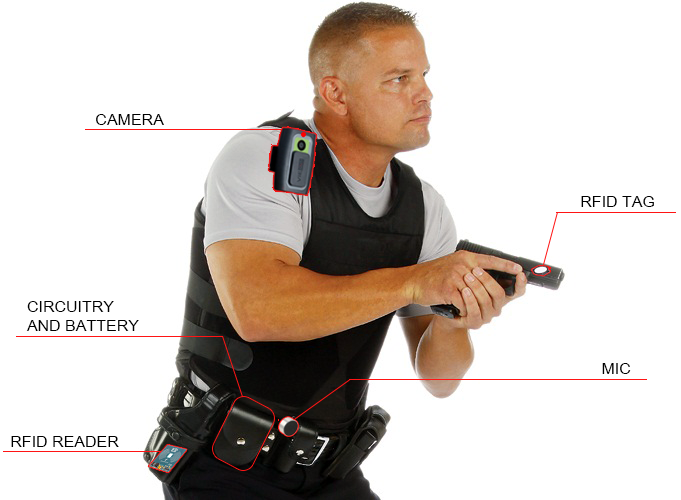
\includegraphics[width=0.9\textwidth]{installation}
    \caption{Overview of Installation}
    \label{fig:installation}
\end{figure}

At the design expo, we demonstrated our project, shown in Figure
\ref{fig:installation}.  Our project is a self-contained, enclosed product
which wirelessly sends camera footage to a laptop at about 1 \gls{fps}. The
product saved camera footage to a \gls{sd} card at a more reasonable 10
\gls{fps}.  The success of this project was in question until nearly the very
end, due to the fact that the \gls{usb} protocol was a much heartier challenge
than originally anticipated. The team met most other milestone objectives with
flying colors. Given this, and the fact that the final product was what we had
proposed (even with some weaker specifications), our project should be deemed a
success and we are happy with the result.

\section{Description}
Every year around 500 people are killed by law enforcement personnel, and many
people are wondering how many of these deaths were justified. One classic way
to ensure that all protocols were being followed has been a police body camera.
However, these are often expensive (\$800 - \$1200 each\cite{cam}) and have
serious privacy concerns for the police officers. If the body cameras are
always on, it might record personal moments that do not need to be seen.
However, if we give the officer a way to turn it on and off, police may tamper
with evidence that could convict them. Benson discusses the various incentives
at work that determine which arrests police are likely to
make\cite[ch.~6]{enterprise_of_law}; similarly, police have an incentive to use
their weapons to stay alive often since they are rarely prosecuted in cases in
which they use lethal force\cite{no_conviction_1,no_conviction_2}. This is not
to say that police officers are bad, but these incentives can be very strong
and may override their sense of duty.

\subsection{Objectives}
When purchasing body cameras, police departments must analyze the costs and
benefits.  The costs of available systems is high; in addition to the high cost
of current units\cite{cam}, storing the amount of footage from body cameras
that are always on represents a significant challenge\cite{store1,store2}. In
addition, many officers fear for their privacy\cite{officer_privacy}. Since the
camera knows when the officer is in danger, backup may be automatically
dispatched before the officer has time to call for it. Finally, a police
department may purchase third-party streaming attachments to stream video to a
third-party cloud system to minimize liability and to ensure the public that
corruption is not likely\footnote{We have not seen any articles on this
concept, although contracting liability to a third party is common.}.  Our
product, shown in Figure \ref{fig:installation}, currently fulfills all of the
above objectives at a prototype level.  It will be priced in the same range as
currently available body cameras, but increases the safety of both officers and
the public while reducing costs.

\subsection{System Description}
An overview of our product is shown in Figure \ref{fig:system_description}.

\begin{figure}[h]
    \centering
    \includegraphics[height=0.5\textheight]{sys_desc}
    \caption{System description}
    \label{fig:system_description}
\end{figure}

\subsection{Trigger System}
\label{sec:sys_trigger}

\begin{figure}[h]
    \centering
    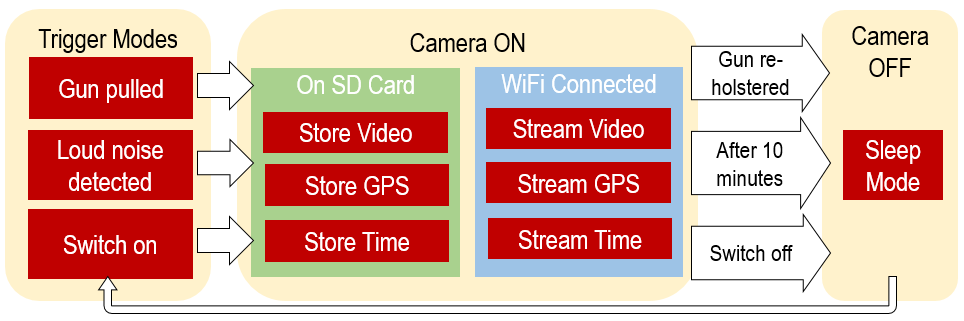
\includegraphics[width=0.9\textwidth]{trigger_flow}
    \caption{Trigger flow}
    \label{fig:trigger_flow}
\end{figure}

The trigger subsystem, shown in Figure \ref{fig:trigger_flow}, consists of the
hardware and software used to process our triggers and send an interrupt to the
TIVA to begin or end recording. The MSP430 takes in a comparator line that
determines the microphone level, an RFID radio card present line, and a manual
switch and determines when to wake the TIVA based on those inputs.

\subsection{Video System}
\label{sec:sys_video}
The video subsystem consists of the hardware and software used to capture video
from a source and send it to various sinks. The source of the video is any
camera that complies with the \gls{uvc} standard. There are currently two
implemented sinks: an on-board \gls{sd} card and streaming to a base station
over Wi-Fi. The larger of the two onboard processors, a TIVA, manages the
transfer of video from source to sinks. The flow of video through the system is
shown in Figure \ref{fig:video_flow}.

\begin{figure}[h]
    \centering
    \includegraphics[width=0.9\textwidth]{subsys_video}
    \caption{Video subsystem}
    \label{fig:video_flow}
\end{figure}

Currently, the driver that handles the video source is compatible with and aims
to fully comply with versions 1.1 and 1.5 of the \gls{uvc}
standard\cite{uvc_standard_11,uvc_standard_15}. The driver supports both a raw
video format\footnote{Specifically the YUY2 encoding} and the MJPEG format. In
order to obtain the highest-quality video at the lowest bandwidth, the driver
prefers MJPEG over raw. In order to choose a resolution, the driver is
initialized with a target bandwidth and then chooses a frame size that will be
as close to that bandwidth as possible without exceeding it. The driver
initialization function declaration is shown in Appendix
\ref{app:software_interfaces}.

The TIVA processor is triggered on by the trigger system, which is described in
Section \ref{sec:sys_trigger}. Once triggered, the TIVA opens connections to
the attached camera, the on-board \gls{sd} card, and the base station via the
Wi-Fi chip. As video data flows in from the camera, the \gls{uvc} driver uses
three callbacks to announce the start of a frame, the data in a frame, and the
end of a frame. Using those callbacks, the video data is both written to the
\gls{sd} card and streamed to the base station.

Our SD card writer is a modified SPI driver that runs through a library called
FatFS. This formats the SPI messages to open files and write to those files with 
relative ease. Our implementation takes the frame that is received from the USB
and writes it to a file in plaintext. From there we can use a similar implementation
on our base station as the WiFi receiver to display the frames with a small delay
inbetween to simulate frame rate. 

The Wi-Fi streaming is comprised of two components; a CC3000 chip that handles
the wireless connection on the body camera system, and a base station that runs
on a computer. The CC3000 streams video data using the \gls{udp} protocol to
the base station, using the proprietary packet format shown in Table
\ref{tab:packet_format}.  The base station receives the video packets, combines
the various chunks in the correct order, and both saves to a hard drive and
displays the video on-screen.

\begin{table}[h]
    \centering
    \caption{Body Camera Streaming Protocol}
    \begin{tabular}{lrr}
        \textbf{Field} & \textbf{Offset} & \textbf{Size (bytes)}\\
        length & 0 & 2\\
        ID & 2 & 1\\
        type & 3 & 1\\
        offset & 4 & 4\\
        data & 8 & length\\
    \end{tabular}
    \label{tab:packet_format}
\end{table}

By saving locally, our product provides resiliency. When a network is not
available, all video data is still saved. It is impossible to destroy the
evidence by jamming the wireless network signal, so even extremely resourceful
criminals and/or very electrically noisy environments will not prevent evidence
from being gathered. By streaming data to a police department or third party
network, our product increases the safety of all parties involved and provides
redundancy to reduce the chance of evidence destruction. The safety of the
parties involved in a violent situation is increased because the police
department knows as soon as an officer enters a violent situation. Backup may
be dispatched without the officer having to request it; in cases where an
officer unknowingly walks into a dangerous situation, this feature is
life-saving.

\subsection{Power System}
Our system is designed to use as little energy as possible by removing power to
all video-related subsystems until video needs to be recorded. The video
subsystem consists of a Texas Instruments TIVA
microcontroller\cite[p.~1880]{tm4c1294ncpdt}, a Texas Instruments CC3000 Wi-Fi
chip\cite[p.~6]{cc3000}, an SD card\cite[p.~19,23]{sd_standard}, a EM-506 GPS
unit\cite[p.~10]{em506}, and a USB camera\cite[p.~245]{usb_standard}. These
parts draw the majority of the power, totalling 4290.4 mW in the worst case.
The rest of the system draws a relatively small 131.4 mW. The individual worst
case power draws are given in Table \ref{tab:worst_case_power}.

% TODO Cite the specification sheets
\begin{table}[h!]
    \centering
    \caption{Worst Case Power Consumption}
    \begin{tabular}{lrrr}
        \textbf{Device} & \textbf{Voltage (V)} & \textbf{Current (mA)} & \textbf{Power (mW)}\\
        TIVA & 3.3 & 133.4 & 440.2\\
        Camera & 5.0 & 500.0 & 2500.0\\
        GPS & 5.0 & 55.0 & 275.0\\
        Microphone & 3.3 & 0.5 & 1.0\\
        RFID Reader & 3.3 & 35.0 & 115.5\\
        SD Card & 3.3 & 100.0 & 330.0\\
        MSP430 & 3.3 & 4.5 & 14.9\\
        CC3000 & 3.6 & 207.0 & 745.2\\
        \hline
        \textbf{Totals} & & & \textbf{Power (mW)}\\
        Idle & & & 131.4\\
        Recording & & & 4421.8\\
    \end{tabular}
    \label{tab:worst_case_power}
\end{table}

In an 8 hour police shift, our device can record up to one half hour of video,
requiring approximately 13.65 Wh of energy. A battery with \textasciitilde{} 20
Wh has been chosen for overhead and to deal with wear in production use. A
lithium-polymer battery was chosen due to the high energy density and ability
to recharge. Lithium-polymer batteries can be dangerous, especially when
exposed to forceful strikes; a tough battery case will mitigate this danger.

\subsection{Mechanical Design}
The mechanics of this design revolve around one enclosure that contains the PCB
that houses the MSP430, GPS, RTC, RFID reader, an exposed switch, and a
microphone. The RFID reader will have an antenna coming out of the enclosure
that will be mounted on the holster. This enclosure will also contain a TIVA
with an attached WiFi radio, which will also have an externally mounted
antenna. The camera will be mounted on the shoulder of the officer and will be
connected to the enclosure via a USB cable, as the camera solution we have is
USB compatible. The camera will also have an enclosure that allows it to
comfortably be mounted to the officer's shoulder. All connections and the
protocols they use can be found in the diagram above.

Another mechanical design feature is the size limitations we will run into.
However, officers already carry weapons as well as radios on their belt, so
anything we add to the belt will not be too much for the officer as long as it
is not big enough to be physically intrusive. However, sticking to just a
camera mounted on the shoulder is key, because something heavy on a shoulder
could knock his aim off and potentially put the officer in a dangerous
situation. 

\subsection{Conclusion}
Our project proposes an optimal scheme to satisfy questions of unethical
conduct by police officers. Even though police officers maintain the right to
apprehend suspects by force, many suspect officers of abuse of their power.
Righteousness of the officers’ actions can not be judged without tangible
evidence of incidents. Having videos recorded only when an incident occurs will
provide tangible evidence to judge whether officers’ actions were just, without
violating officers’ privacy. One of the difficulties is that it is difficult to
precisely distinguish a moment to start recording a video well enough to
encompass whole situation. Achieving live streaming is optimal but will be
challenging to get done in the given scope of the project. However, once our
proposed function is achieved, it will open many possibilities to extend its
uses and functionalities. When successful, this project will provide optimal
functionality for the use of a wearable body camera in a tactical application. 

\section{Milestones, Schedule, and Budget}
Most of this project was on schedule from the beginning. The only problem we
really ran into was getting our final piece of the puzzle in place: decoding
our video. Once we that was working, the remainder of the project was quickly
integrated and a full feature prototype was able to be tested. Our original
schedule is shown in Appendix \ref{app:gantt}. All deadlines were met except
for the Camera Driver, which was not in testing until late November and
finished until early December.

Our original budget was around \$312.93 and we spent \$884.91 % TODO

\subsection{Milestone 1}
\subsubsection{GPS and RTC Implementation and Verification}
Getting an early GPS parser was one of the easier parts of the project, while
it was also one of the more unnecessary parts for a working demo. GPS was done
early, but it turned out not to be very vital to the success of the project.

\subsubsection{Audio and Manual Trigger Implementation and Verification}
This was a very early victory that helped the trigger side of our project get
done as quickly as it did. We had a working prototype for the MSP430 trigger
processor about a week before the first milestone and we had a final version a
few weeks later, which ensured that once we got all of the TIVA video
processing done, we could easily integrate the two parts together.

\subsubsection{Wi-Fi Testing}
Originally we had a UART-based WiFi module that did not have a great datasheet
or any sort of support on the internet. With this in mind and the fact that it
seemed to overheat easily, we looked for a quick replacement. What we found was
the CC3000, which boasted a 4Mbps data transfer rate over TCP. Having a little
bit of background in networking, we figured UDP would be even faster so we
locked this in as our choice and had a quick demo in which we sent packets over
to a host computer.

\subsubsection{RFID in Development}
We managed to find a reliable RFID radio that had a card-present line which
suited our needs very well. The development on this part was basically
nonexistent, so that the trigger processing reached completion even quicker. We
had the RFID part completely working by the time this milestone came around.

\subsubsection{Video Data Encoded}
Video data was the slowest part of our project to develop, since writing a USB
device driver is no small task. We did not manage to see video until around a
month and a half after the first milestone. This milestone portrayed both our
hearty ambition and innocent ignorance.

\subsection{Milestone 2}
\subsubsection{Working Full-Featured Prototype}
This was definitely the issue that kept us behind on our project. We did not
have verified data by the second milestone, so it was difficult to test
anything. Our team had all of the other parts done, like a WiFi driver that
could send at a reasonable speed and all of the trigger processing in its final
state, but without being able to see video we were not sure whether or not the
project would be completed on time.

\subsubsection{PCB is Shipped}
We overestimated the time required to get a PCB out so by the time the second
milestone came around we had already populated our PCB and begun testing.
Luckily for us, we had plenty of time to order a second version of a PCB which
addressed problems we had like an incorrect crystal, an unorderable SD card
reader, and a few small on-board revisions we needed to make. Getting this done
as early as we did definitely helped us stay on track.

\subsubsection{Enclosure Designed}
This goal was also underestimated. Our team had a first version enclosure
printed that helped us form the next and final version that we have on the
final prototype. Having this milestone completed also helped us stay on track.

\subsection{Budget and Bill of Materials}

% TODO budget goes here


\section{Lessons Learned}
When we reflect on the outcome of our project, there are a few points which we
wish we would have known before the project started, and so are points we have
since learned. 

The first mistake our group made was to create specifications and requirements
without first researching to a point where we would be able to realistically
quantify them. Instead, we had a tendency to create requirements based on the
ideal case - what we thought would be nice to have or a good goal to have
before us. This lack of research is reflected in the part choices we made (i.e.
the CC3000), and really propagated throughout our entire project. The cliché
``measure twice, cut once'' comes to mind with regards to this situation.

Also, we learned that most of tasks require steep learning curve, and it is
very hard for other members to participate in tasks that has already made
significant progress. Other members trying to help incomplete tasks after their
given tasks had difficulty in catching up the already made progress but time
was limited for the original member of the task to walk through the progress
that he had already made. This resulted in some of team members doing more
works than the others. We learned that it is important to distribute works
correctly and that all team members keep track of each other's tasks.

An element of our project that really went well was the choice of development
board and process we used to convert development board to custom circuit board.
The development board had a great deal of pinouts and functionality that made
the schematic creation process easy. We were able to test on the development
board using the exact same pins and peripherals that would later be used on the
PCB. This meant that once the hardware was ready and correct, the software
worked almost immediately, with little software debugging.

The design of the enclosure was an afterthought, and the project appeared to be
poorly integrated because of this. The enclosure was bright blue, and very
noticeably duct-taped to the officer's holster during the design expo. Another
reason for the poor enclosure design was that the PCB was routed with the sole
constraint that it should work, and no thought was given to a good form factor
for packaging. In the future, care should be taken to route the circuit
board(s) in such as way as to integrate well with the officer's belt and
holster.

Overall, if we could send a message to ourselves before the project started, it
would be to continue to work hard from the beginning and to not underestimate
the complexity from USB. Our group did a great job working a steady,
substantial amount throughout the life of the project. We did end up having to
work more towards the end of the project, but this was because we had
underestimated the amount of work the USB driver would require, and this
delayed all parts, including work on the PCB. So, if we could go back and
increase work on this portion of our project in the beginning, or avoid
undertaking that monstrous task altogether.

\subsection{Individual Lessons Learned}
Alec learned about writing a USB device driver, and choosing video formats
based on bandwidth constraints. He also experienced soldering a TQFP with more
than 64 pins for the first time, and learned from Yitian how to use flux to fix
solder bridges. He also learned a bit about designing a network protocol.

Alex learned about researching parts. This involved not only finding a part
that meets the requirements of the project but also researching different
sources for the same part. This was learned the hard way by choosing a WiFi
module that has been retired and is no longer supported by TI, something that
made finding resources much more difficult. He also learned about PCB
verification and how to make sure individual parts of the PCB are working while
not having the others functional. 

Jacob learned about designing a PCB using Eagle. This involved coordination
with each team member to discuss options regarding schematic (pin selection)
and layout considerations. After fabrication, he was forced to learn a great
deal about debugging hardware, including what not to do (i.e. shorting pins
with bad probes).

Jiqing got familiar with the process flow of programming in Code Composer
Studio from TI and the 3D design by using Solidworks. He learned about the
working principle of reading from and writing to a SD card via SPI
communication and how each individual function got integrated in a whole
system. He also learned about using Logic Analyzer to debug and asking TI
supporting team online for help. He worked with Alec on establishing a USB
device driver in the beginning of the project and learned its working principle
with the help of Alec and examples from documents.

Yun learned about an overall real-application design process that includes PCB
design and manufacturing, 3D design and printing, and group coordination
through Github. Also, he learned about video protocol and its encoding and
decoding methods.

\section{Contributions}
A summary of individual contributions is given in Table
\ref{tab:individual_contrib}, and details are given below.

\begin{table}[h]
    \centering
    \caption{Individual team member contributions}
    \begin{tabular}{llr}
        \textbf{Team Member} & \textbf{Summary of Contribution} & \textbf{Effort}\\
        Alec Ten Harmsel & UVC driver, base station, power analysis & 25\%\\
        Alex LaBerge & Wi-Fi driver, \gls{gps}, sleep mode, \gls{pcb} verification & 25\%\\
        Jacob Perrin & \gls{pcb} design and assembly, group coordination & 20\%\\
        Jiqing Jiang & \gls{sd} card driver, \gls{uvc} driver, enclosure design, poster design & 15\%\\
        Yun Chan Han & Trigger circuitry and software, enclosure design, poster design & 15\%\\
    \end{tabular}
\end{table}

Alec was responsible for the USB Video Class device driver. This driver parsed
the configuration of the connected USB camera, determined the optimal format
and video size based on bandwidth constraints, and then configured the camera.
After camera configuration, the driver also implemented the “top” side of an
interrupt-based video capture solution. In addition, Alec wrote the base
station code, which listened on the network for video broadcasted by the body
camera system, converted it to a reasonable format with OpenCV, and displayed
it with the Qt Toolkit. Finally, Alec was responsible for the power system
design and reviewing the circuit schematics and layouts produced by Jake.

Alex was responsible for the main control loop for the TIVA recording software,
which included integrating his WiFi and GPS drivers in with Alec's USB driver.
He debugged the SD card implementation and formatted Jiqing's driver to work with
the pins that the PCB used, as well as integrated that feature into the control loop. 
He optimized the TI library for the WiFi module to get the fastest throughput
possible on the CC3000 by removing unnecessary delays and making the sockets
nonblocking. Alex also wrote the first iteration of base station socket code
which received the data streamed from the TIVA, which was later improved by
Alec. Finally, Alex was responsible for verifying the components on the PCB
worked and debugging the issues that arose.

Jacob was primarily responsible for all activities related to the hardware, and
specifically the PCB. As such, he designed the schematic and layout for the
PCB. The PCB was designed before most parts of the prototype had been finished,
or even begun. As such, this took a good deal of effort and care (there were
still small errata on the final version of the PCB). He also took part in the
assembly of four different PCB boards. Additionally, Jacob was responsible for
coordinating group activities and communication with outside parties. This
includes getting sponsored by Advanced Circuits as well as doing any
miscellaneous grunt work that the group came across through the life of the
project.

Jiqing was responsible for the implementation of saving video data in a micro
SD card on TM4C1294NCPDT and the enclosure design in Solidworks. He also helped
to debug for system integration and checking PCB design when things did not
work. He also worked with Alec on the USB video class device driver and
designed the poster.

Yun was responsible for the hardware and software of triggering portion of the
project. He designed the schematic of a circuitry that takes analog and digital
inputs from a switch, a microphone, and a RFID reader. The circuitry he
designed was adjustable in that the noise level can be controlled externally.
Then he designed the triggering logic to start and end the video recording on
MSP430. He also designed a tamperproof enclosure that protects a USB cable
connection and a SD card from users. He designed the poster for design expo as
well.

\section{Cost of Manufacture}
Our total estimated cost of manufacturing is \$120 for any quantity greater
than 150. This seems like a very reasonable number given the price of the parts
listed above. This quote includes the WiFi breakout and RFID module. The only
additional pieces of hardware that would be needed in order to make this quote
a complete package would be the camera, battery, and enclosure. These items
would likely bring the price to manufacture this item to somewhere closer to
\$200-\$250. Given that we would need to rethink some partitions of this project,
most important among these being WiFi bandwidth and microprocessor processing
power, this number does appear to be very rough. However, with this cost of
manufacturing, such a product could be very competitive in this market, where
prices can often be found near the \$1000 range.

\section{Parts}
% TODO Table of parts with prices
% TODO Table of part prices for mass production

\newpage

\bibliographystyle{plain}
\bibliography{references}

\newpage

\appendix

\begin{landscape}
    \section{Gantt Chart}
    \label{app:gantt}
    \thispagestyle{empty}

    \begin{figure}[h!]
        \centering
        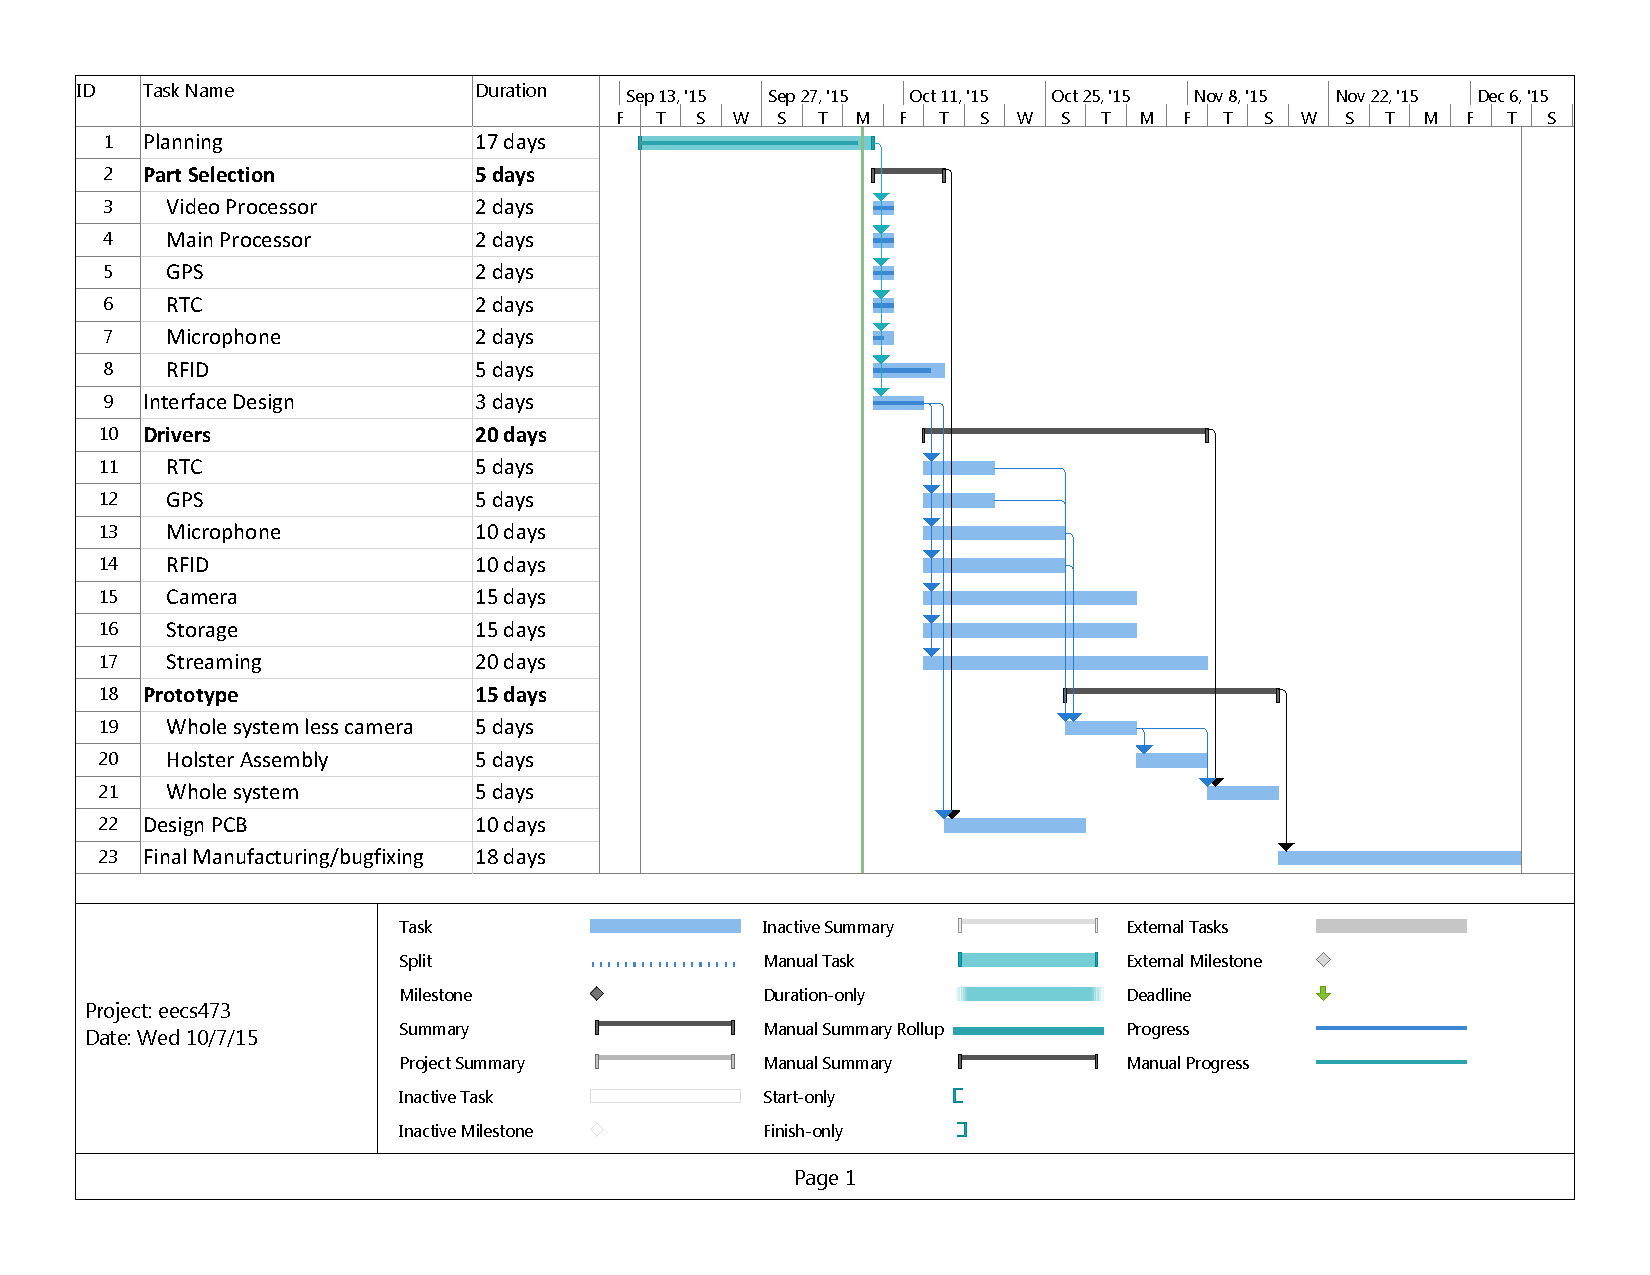
\includegraphics[width=1.1\textwidth]{gantt}
        \caption{Gantt chart}
        \label{fig:gantt}
    \end{figure}
\end{landscape}

\newpage

\section{Software Interfaces}
\label{app:software_interfaces}
% TODO

\subsection{UVC/Camera Interface}
\lstinputlisting{uvc.h}

\newpage

\subsection{Network Interface}
\lstinputlisting{network.h}

\newpage

\subsection{GPS Interface}
\lstinputlisting{gps.h}

\newpage

\subsection{Trigger Interface}
\lstinputlisting{trigger.h}

\newpage

\section{PCB Design and Layout}

\begin{figure}[h]
    \centering
    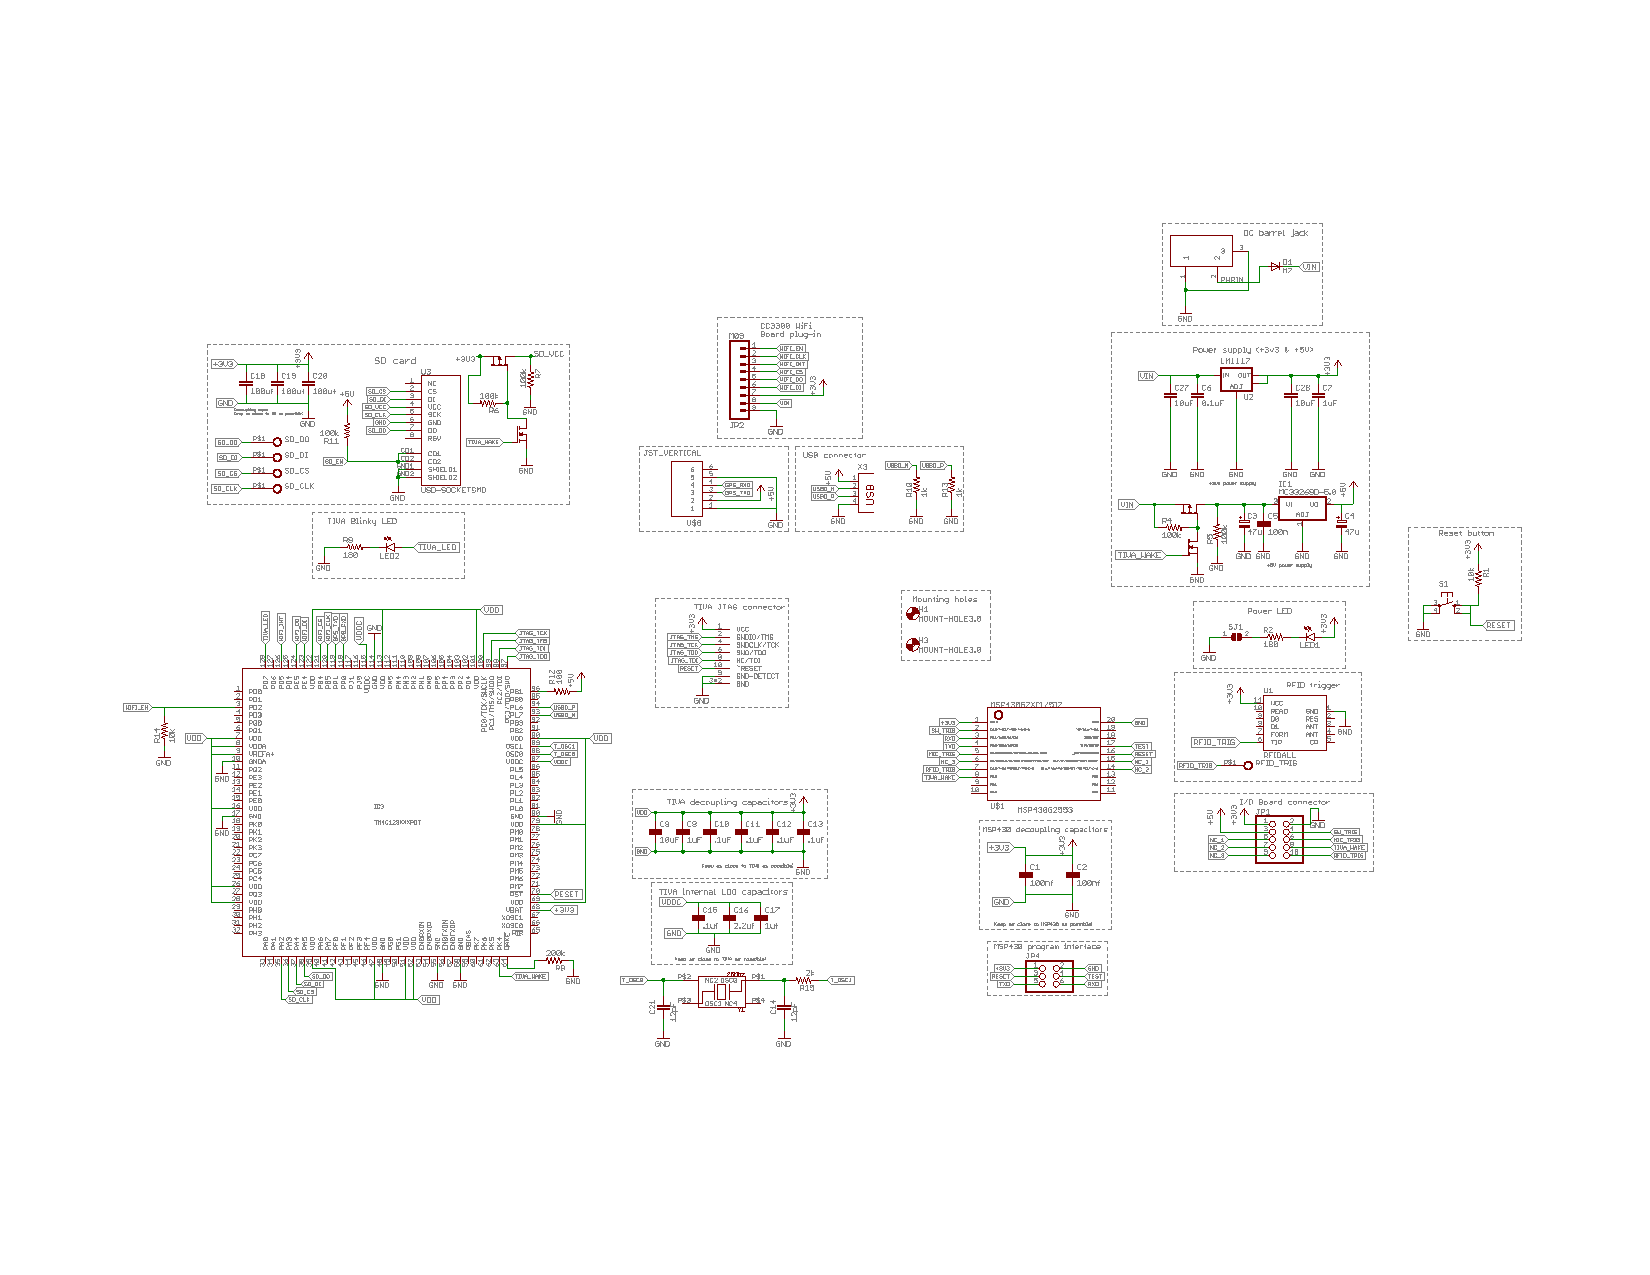
\includegraphics[angle=-90,width=0.99\textwidth]{BodyCamBoard_sch}
    \caption{Main board schematic}
\end{figure}

\begin{figure}[h]
    \centering
    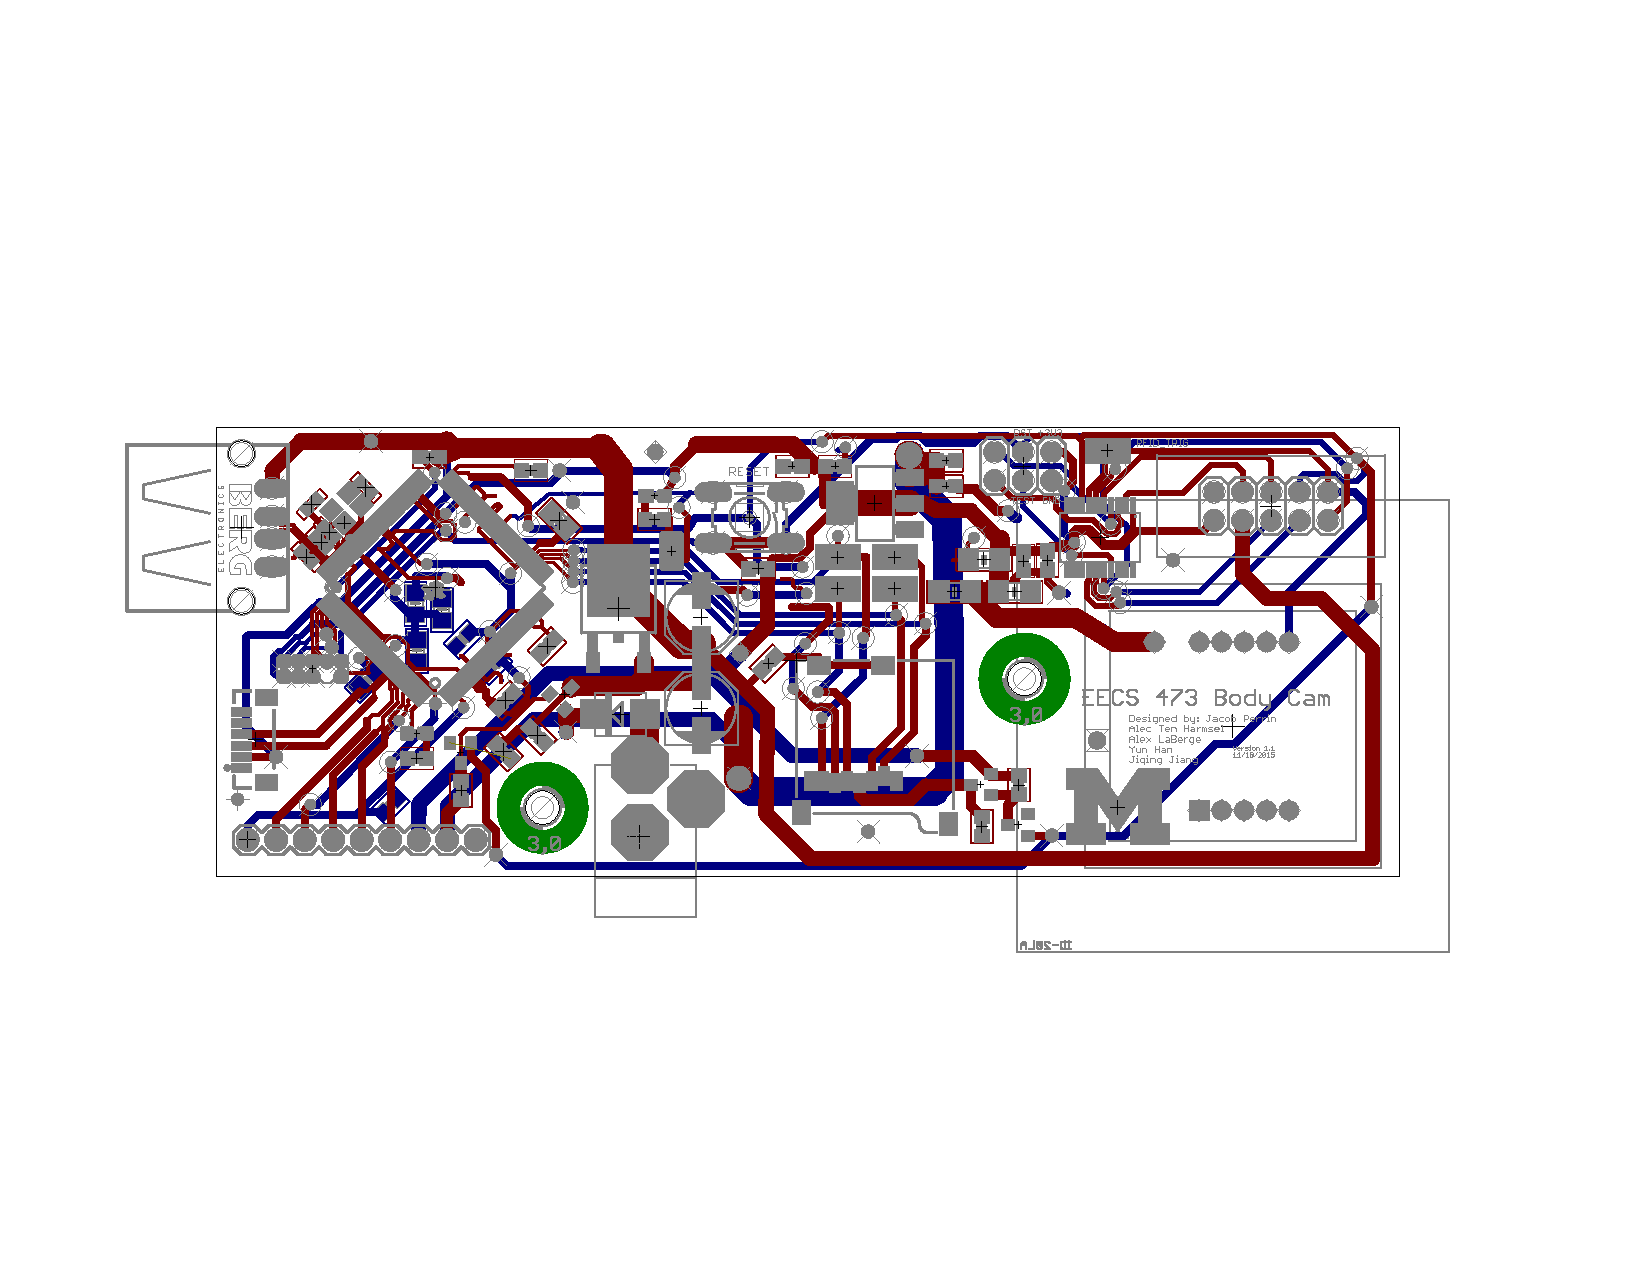
\includegraphics[angle=-90,width=0.99\textwidth]{BodyCamBoard_brd}
    \caption{Main board layout}
\end{figure}

\begin{figure}[h]
    \centering
    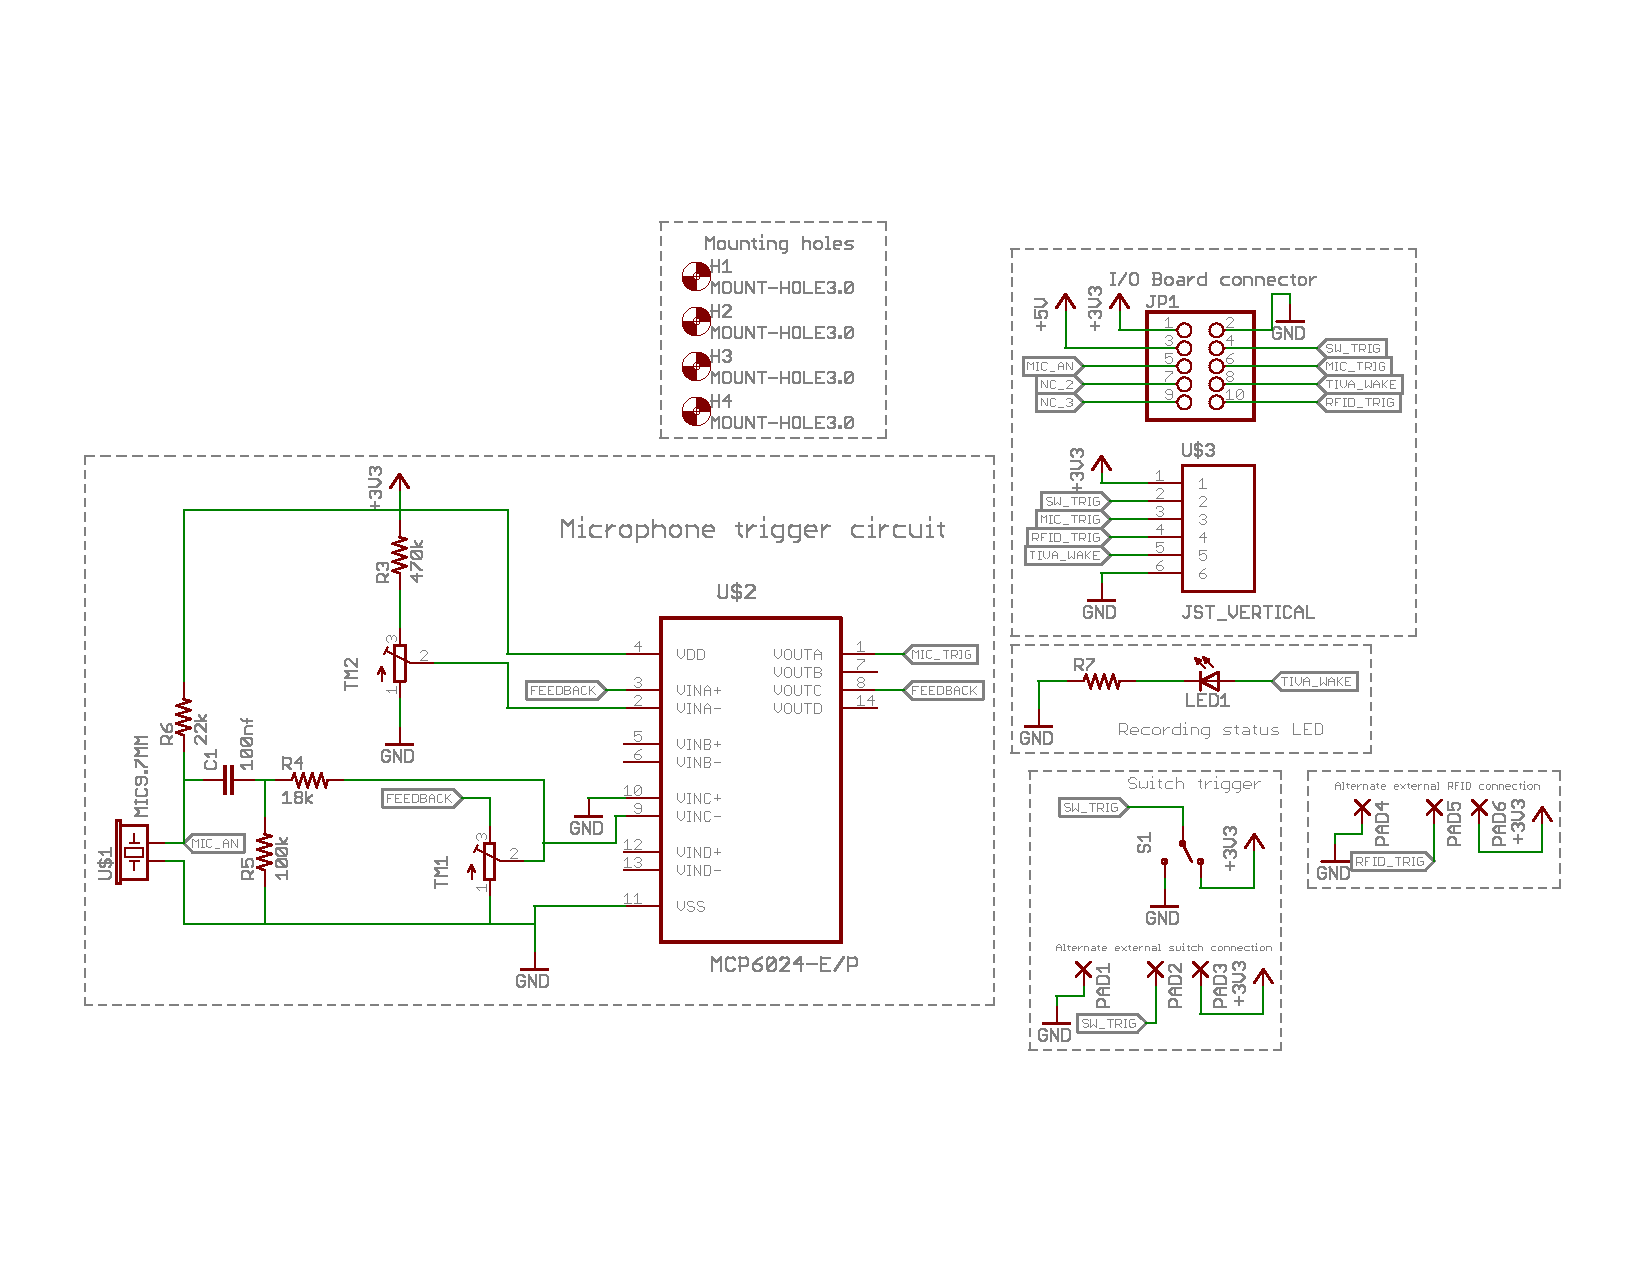
\includegraphics[angle=-90,width=0.99\textwidth]{IOBoard_sch}
    \caption{I/O board schematic}
\end{figure}

\begin{figure}[h]
    \centering
    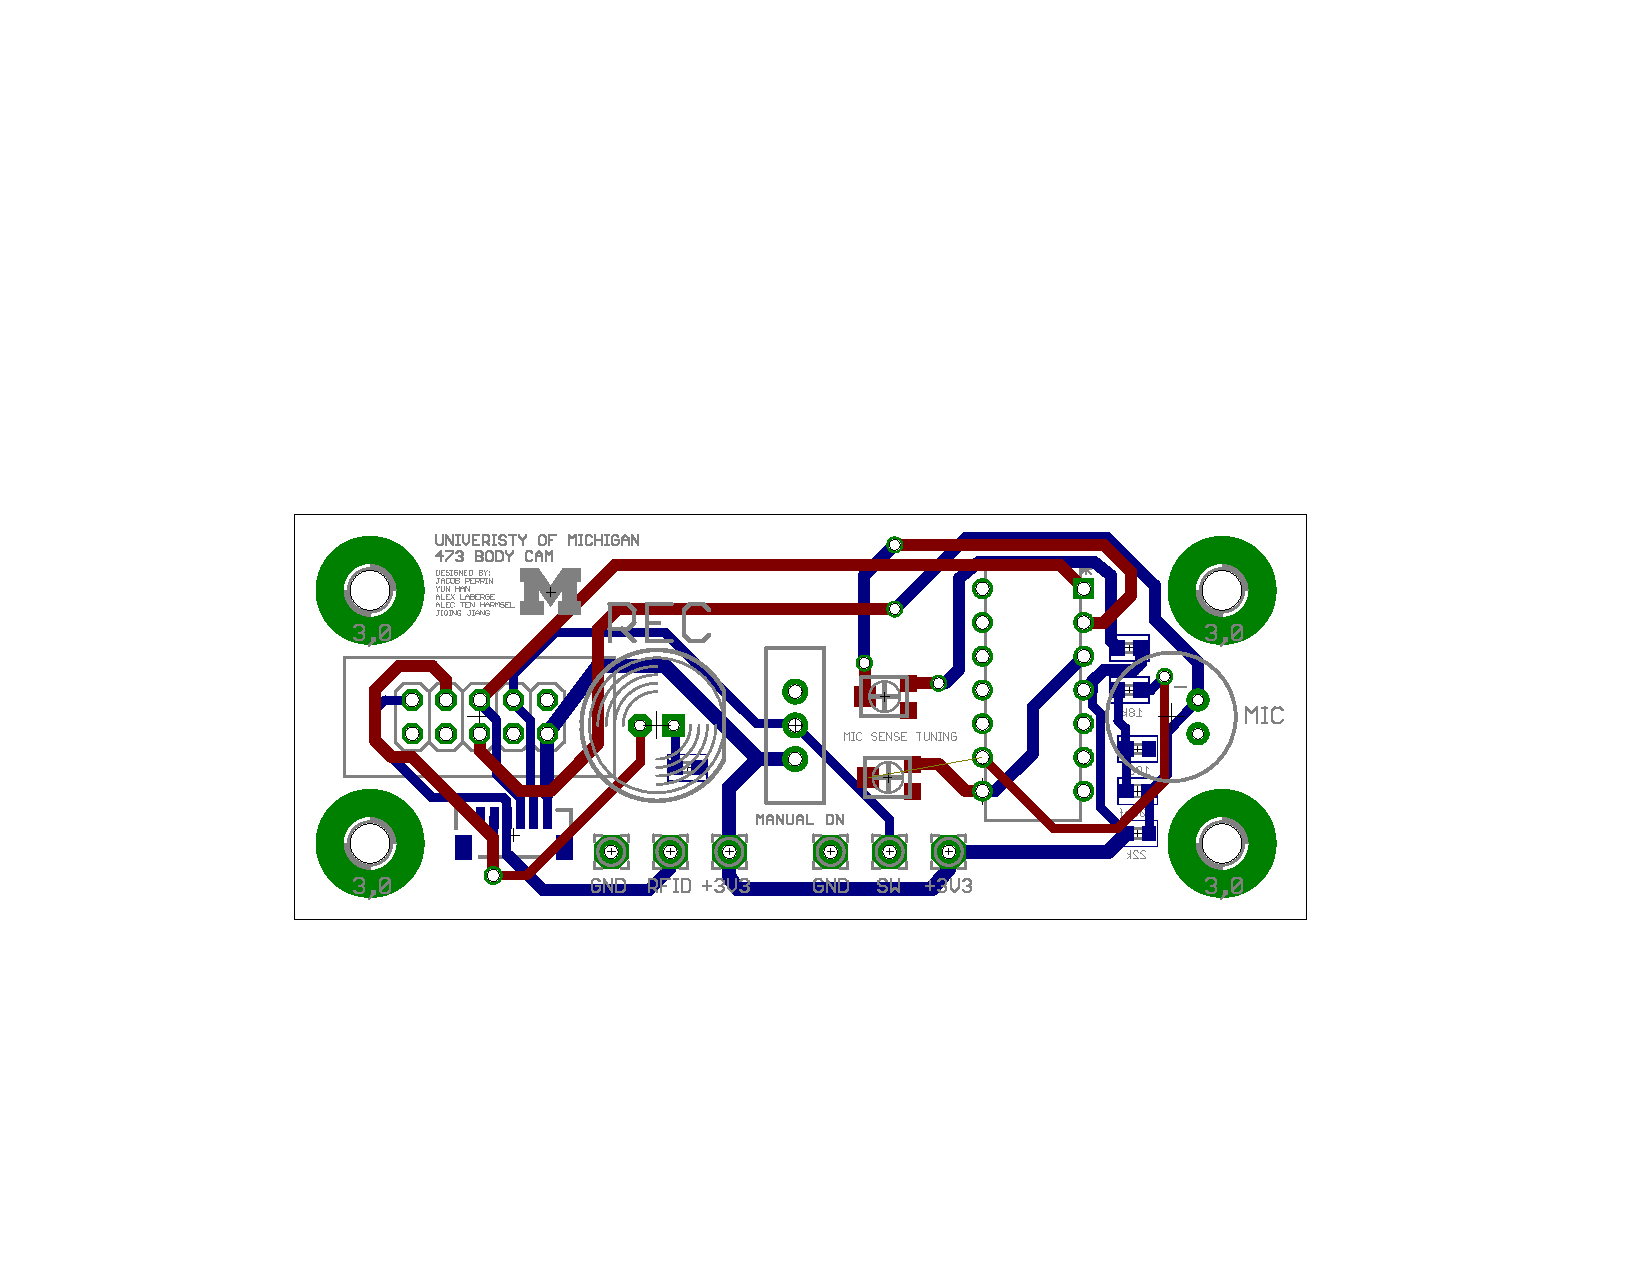
\includegraphics[angle=-90,width=0.99\textwidth]{IOBoard_brd}
    \caption{I/O board layout}
\end{figure}

\end{document}
